\documentclass[fleqn]{article}
\oddsidemargin 0.0in
\textwidth 6.0in
\thispagestyle{empty}
\usepackage{import}
\usepackage{amsmath}
\usepackage{graphicx}
\usepackage{flexisym}
\usepackage{amssymb}
\usepackage{bigints} 
\usepackage[english]{babel}
\usepackage[utf8x]{inputenc}
\usepackage{float}
\usepackage[colorinlistoftodos]{todonotes}

\definecolor{hwColor}{HTML}{AD53BA}

\begin{document}

  \begin{titlepage}

    \newcommand{\HRule}{\rule{\linewidth}{0.5mm}}

    \center



    \textsc{\LARGE Arizona State University}\\[1.5cm]

    \textsc{\LARGE Mathematical Methods For Physics II }\\[1.5cm]


    \begin{figure}
      
\includegraphics[width=\linewidth]{asu.png}
    \end{figure}


    \HRule \\[0.4cm]
    { \huge \bfseries Homework Fifteen}\\[0.4cm] 
    \HRule \\[1.5cm]

    \textbf{Behnam Amiri}

    \bigbreak

    \textbf{Prof: Cecilia Lunardini}

    \bigbreak


    \textbf{{\large \today}\\[2cm]}

    \vfill

  \end{titlepage}

  \begin{enumerate}
    \item Evaluate the following definite integral: 
    $$\int^{2\pi}_0 \frac{d\theta}{p^2 -2p \cos\theta+1}~$$ 
    where $-1<p<1$.

      \textcolor{hwColor}{
        $
          \begin{cases}
            z=e^{i \theta} \longrightarrow dz=iz d\theta
            \\
            \\
            e^{i \theta}+e^{-i\theta}=\left[cos(\theta)+i sin(\theta)\right]+\left[cos(\theta)-i sin(\theta)\right] \Longrightarrow cos(\theta)=\dfrac{1}{2} \left(e^{i \theta}+e^{-i \theta}\right)=\dfrac{1}{2} \left(z+\dfrac{1}{z}\right)
          \end{cases}
          \\
          \\
          \\
          I=\bigints\limits_{0}^{2 \pi} \dfrac{d\theta}{p^2-2p cos(\theta)+1}
          \\
          \\
          =\bigints\limits_{0}^{2 \pi} \dfrac{\dfrac{dz}{iz}}{p^2-2p \left[\dfrac{1}{2} \left(z+\dfrac{1}{z}\right)\right]+1}
          \\
          \\
          =\dfrac{1}{i} \bigints\limits_{0}^{2 \pi} \dfrac{dz}{zp^2-p\left(z^2+1\right)+z}
          \\
          \\
          =-i \bigints\limits_{0}^{2 \pi} \dfrac{dz}{zp^2-p\left(z^2+1\right)+z}
          \\
          \\
          =-i \bigints\limits_{0}^{2 \pi} \dfrac{dz}{(p-z)(zp-1)}
        $
        \\
        \\
        What we ended up with is a function that has two poles 
        \\
        \\
        $
          \begin{cases}
            z=p
            \\
            z=p^{-1}
          \end{cases}
        $
        Based on the two poles we have the two scenarios: \\
        \\
        \\
        \\
        \textbf{(A) ~ $|z|>1$}
        \\
        \\
        $
          Res(f(p^{-1}))=\lim\limits_{z \to p^{-1}} \dfrac{i (z-p^{-1})}{p(z-p)(z-p^{-1})}=i\dfrac{1}{1-p^2}
        $
        \\
        \\
        \rule{15cm}{1pt}
        \\
        \\
        \textbf{(B) ~ $|z|<1$}
        \\
        \\
        $
          Res(f(p))=\lim\limits_{z \to p} \dfrac{i (z-p)}{p(z-p)(z-p^{-1})}=\dfrac{i}{p^2-1}
        $
        \\
        \\
        \\
        I=$
          \begin{cases}
            I_A=2 \pi i Res(f(p^{-1}))=\dfrac{2 \pi}{1-p^2} ~~~~~ \surd
            \\
            \\
            I_B=2 \pi i Res(f(p))=\dfrac{2 \pi}{p^2-1} ~~~~~ \surd
          \end{cases}
        $
      }
    
    \item Evaluate the following integrals:
    \begin{enumerate}
      \item $$ \int^{+\infty}_{-\infty} \frac{ e^{imx}}{1+x^2}dx$$

        \textcolor{hwColor}{
          $
            f(z)=\dfrac{e^{imz}}{(z+i)(z-i)}
          $
          \\
          \\
          thr poles are $i$ and $-i$. \\
          \\
          \\
          $
            Res(f(i))=\lim\limits_{z \to i} \dfrac{(z-i) e^{imz}}{(z+i)(z-i)}=\lim\limits_{z \to i} \dfrac{e^{imz}}{(z+i)}=\dfrac{e^{-m}}{2i}
          $
          \\
          \\
          Now picture a circle centered at the origin with radius $r$. Then we have: \\
          \\
          $
            \oint\limits_{C} f(z) dz=\bigints\limits_{-r}^{r} f(z) dz
            \\
            \\
            2 \pi i ~ Res(f(i))=\bigints\limits_{-r}^{r} f(z) dz
            \\
            \\
            2 \pi i \times \dfrac{e^{-m}}{2i}=\bigints\limits_{-r}^{r} f(z) dz
            \\
            \\
            \\
            \therefore ~~~~ \bigints\limits_{-\infty}^{+\infty}=\dfrac{e^{imx}}{1+x^2} dx=\pi e^{-m} ~~~~ \surd
          $
        }
  
      \item $$ \int^{+\infty}_{0} \frac{ x^2}{1+x^4}dx$$
      
        \textcolor{hwColor}{
          $
            f(z)=\dfrac{z^2}{1+z^4} 
          $
          \\
          \\
          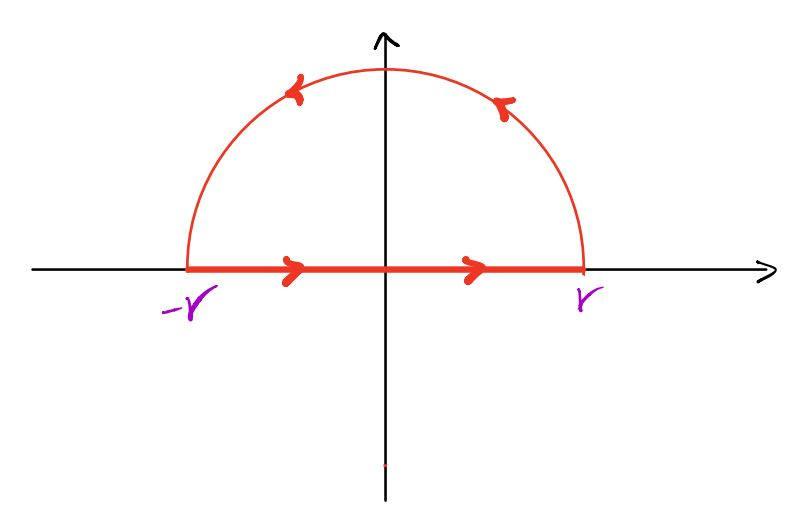
\includegraphics[height=4cm, width=7cm]{Capture.JPG}
          \\
          \\
          Based on $f(z)$ the poles is when $x^4=-1$, hence the poles are $
          \begin{cases}
            e^{i \pi/4}
            \\
            e^{3 i \pi/ 4} 
          \end{cases}
          $
          \\
          \\
          \textbf{(A)}
          \\
          \\
          $
            Res(f(e^{i \pi/4}))=\lim\limits_{z \to e^{i \pi/4}} \dfrac{z^2(z-e^{i \pi/4})}{1+z^4}
            \\
            \\
            =\lim\limits_{z \to e^{i \pi/4}} \dfrac{z^3-z^2 e^{i \pi/4}}{1+z^4}
            \\
            \\
            =\lim\limits_{z \to e^{i \pi/4}} \dfrac{3z^2-2ze^{i \pi/4}}{4z^3}
            \\
            \\
            \\
            \therefore ~~~~ Res(f(e^{i \pi/4}))=\dfrac{1}{4 e^{i \pi/4}} ~~~~ \surd
          $
          \\
          \\
          \rule{15cm}{1pt}
          \\
          \\
          \textbf{(B)}
          \\
          \\
          $
            Res(f(e^{3 i \pi/ 4}))=\lim\limits_{z \to e^{3 i \pi/ 4}} \dfrac{z^2(z-e^{3 i \pi/ 4})}{1+z^4}
            \\
            \\
            =\lim\limits_{z \to e^{3 i \pi/ 4}} \dfrac{z^3-z^2 e^{3 i \pi/ 4}}{1+z^4}
            \\
            \\
            =\lim\limits_{z \to e^{3 i \pi/ 4}} \dfrac{3z^2-2z e^{3 i \pi/ 4}}{4z^3}
            \\
            \\
            \\
            \therefore ~~~~ Res(f(e^{3 i \pi/ 4}))=\dfrac{1}{4e^{3 i \pi/ 4}} ~~~~ \surd
          $
          \\
          \\
          By using the $(24.70)$ equation we have:
          \\
          \\
          \\
          \rule{15cm}{1pt}
          \\
          \\
          $
            \oint\limits_{C} f(z) dz=\bigints f(z) dz+\bigints\limits_{-r}^{r} f(z) dz
            \\
            \\
            \left[2 \pi i Res(f(e^{i \pi/4}))\right]+\left[2 \pi i Res(f(e^{3 i \pi/ 4}))\right]=\bigints f(z) dz+\bigints\limits_{-r}^{r} f(z) dz
            \\
            \\
            \left[2 \pi i \dfrac{1}{4 e^{i \pi/4}} \right]+\left[2 \pi i \dfrac{1}{4e^{3 i \pi/ 4}}\right]=\bigints f(z) dz+\bigints\limits_{-r}^{r} f(z) dz
            \\
            \\
            \dfrac{1}{2} \pi i \left[cos(\pi/4)- i sin(\pi/4)+ cos(3\pi/4)-i sin(3\pi/4)\right]=\bigints f(z) dz+\bigints\limits_{-r}^{r} f(z) dz
            \\
            \\
            \\
            \therefore ~~~~ \dfrac{1}{\sqrt{2}} \pi=\bigints f(z) dz+\bigints\limits_{-r}^{r} f(z) dz ~~~~ \surd
          $
          \\
          \\
          \\
          \\
          When $R \to \infty$, then we have: \\
          \\
          \\
          $
            \bigints\limits_{0}^{+\infty} \dfrac{x^2}{1+x^4} dx=\dfrac{1}{2} \bigints\limits_{-\infty}^{+\infty} \dfrac{x^2}{1+x^4} dx
            \\
            \\
            \\
            \therefore ~~~~ \bigints\limits_{0}^{+\infty} \dfrac{x^2}{1+x^4} dx=\pi \dfrac{\sqrt{2}}{4}
            \\
            \\
          $
        }

    \end{enumerate}
    \item Evaluate the integral:
    $$\int^{+\infty}_{0} \frac{ \sqrt{x}}{1+x^3}dx$$
    (Hint: take inspiration from the example(s) shown in class. ) 

      \textcolor{hwColor}{
        $
          I=\bigints\limits_{0}^{+\infty} \dfrac{\sqrt{x}}{1+x^3} dx
        $
        \\
        \\
        Let $u=\sqrt{x}$ then we have: \\
        \\
        \\
        $
          I=\dfrac{2}{3} \bigints\limits_{0}^{+\infty} \dfrac{1}{1+u^2} du 
        $
        \\
        \\
        Let \textbf{C} be the closed path of the semi-circle of radius \textbf{R} on the upper 
        half of the complex plane along with the real axis traversed counter-clockwise. Then when $R \to \infty$
        the integral along the semi circle goes to 0. \\
        \\
        $
          I=\dfrac{2}{3} \bigints\limits_{C} \dfrac{1}{1+z^2} dz=\dfrac{2}{3} \bigints\limits_{C} \dfrac{1}{(z-i)(z+i)} dz
        $
        \\
        \\
        Note this is not equal to the original integral since as $R \to \infty$ we are left with the integral from
        $-\infty$ to $+\infty$. But we can divide the integral by 2 to solve for the integral from $0$ to $+\infty$.
        \\
        \\
        $
          \dfrac{1}{3} \bigints\limits_{C} \dfrac{1}{(z-i)(z+i)} dz
          \\
          \\
          \\
          \therefore ~~~~ Res(f(i))=\lim\limits_{z \to i} \dfrac{1}{z+i}=\dfrac{1}{2i} ~~~~ \surd
        $
        \\
        \\
        Note: In the interior of \textbf{C} , there is a pole of order 1 at i.
        \\
        \\
        \\
        $
          \Longrightarrow I=\bigints\limits_{0}^{+\infty} \dfrac{\sqrt{x}}{1+x^3} dx
          \\
          \\
          =\dfrac{1}{3} \bigints\limits_{C} \dfrac{1}{(z-i)(z+i)} dz=\dfrac{1}{3} 2 \pi i Res(f(i))
          \\
          \\
          =\dfrac{1}{3} 2 \pi i \times \dfrac{1}{2i}
          \\
          \\
          \\
          \therefore ~~~~ I=\dfrac{\pi}{3} ~~~~ \surd
        $
      }
    
  \end{enumerate}

\end{document}
